\level{2}{Dashboard APS}
	La \insglo{dashboard} è una pagina web generata in automatico dal \insglo{server} \insglo{Norris}. Essa è costituita da più grafici che l'utente finale potrà visualizzare sul proprio \insglo{browser}. Di seguito viene fornito un \insglo{mockup} a scopo esclusivamente illustrativo: questo vuole essere un esempio sul quale basarci una volta che andremo a costruire la \insglo{dashboard}.
	\begin{figure}[H]\centering
        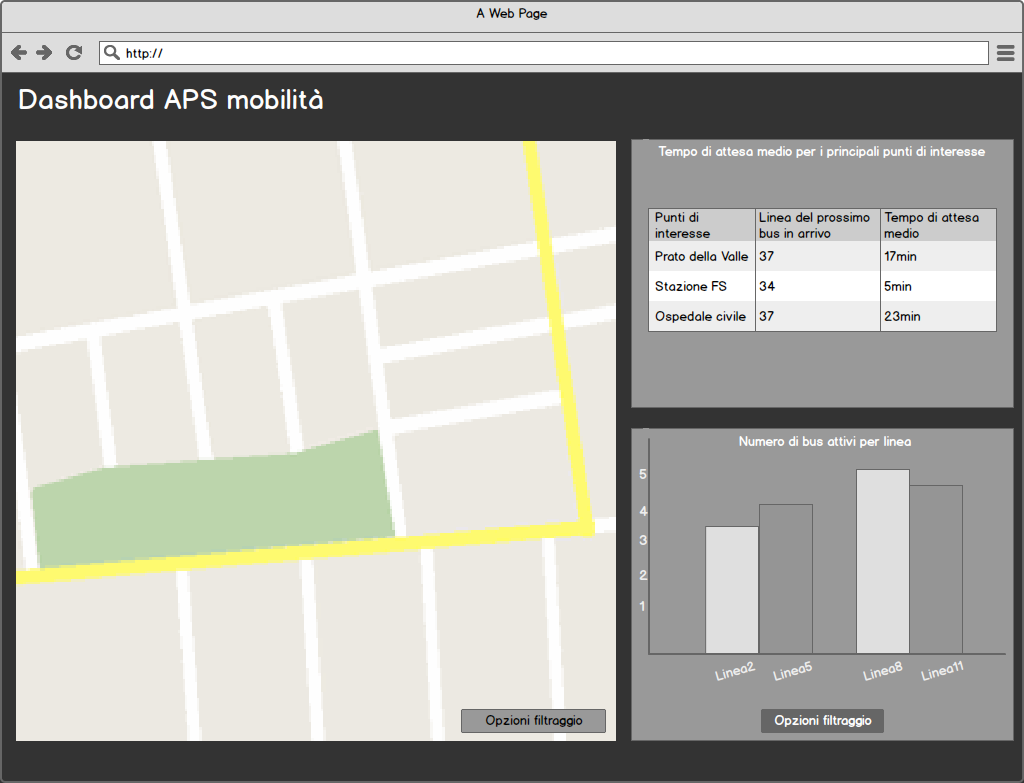
\includegraphics[width=\textwidth]{SpecificaTecnica/Pics/DashboardMockup}
        \caption{Mockup della dashboard APS}
    \end{figure}
    Vengono ora descritti i vari componenti di cui è fatta la pagina, che coincidono con i grafici che sono stati inseriti all'interno del \insglo{mockup} mostrato in precedenza.
    \level{3}{Descrizione delle componenti della Dashboard}
    	\level{4}{Map chart}
    		Tramite questo grafico l'utilizzatore della \insglo{dashboard} è in grado di visualizzare in tempo reale la posizione di tutti i bus attivi nelle varie linee dell'\insglo{APS}. Tale grafico permette inoltre di filtrare le varie linee presenti, in modo tale da visualizzare solo quelle desiderate dall'utente stesso.
    	\level{4}{Table}
    		Tale grafico è dedicato ai punti di maggior interesse di Padova. Esso fornisce all'utente utilizzatore della \insglo{dashboard} il tempo necessario all'arrivo degli autobus in alcune fermate \insglo{APS} molto frequentate. In particolare è possibile visualizzare quanto tempo manca all'arrivo del prossimo autobus in una determinata stazione, e a quale linea il suddetto autobus appartiene.
    	\level{4}{Bar chart}
    		Questo grafico permette all'utilizzatore della \insglo{dashboard} di visualizzare quanti autobus sono attivi su ciascuna linea dell'\insglo{APS}. Egli, inoltre, ha la possibilità di filtrare le varie linee presenti, ossia può scegliere quali sono le linee di cui vuole visualizzare il numero di autobus attivi e quali no.
